\documentclass[conference]{IEEEtran}
\IEEEoverridecommandlockouts
\usepackage{cite}
\usepackage{amsmath,amssymb,amsfonts}
\usepackage{graphicx}
\usepackage{booktabs}
\usepackage{array}
\usepackage{xcolor}
\usepackage[hidelinks]{hyperref}
% Auto-generated by experiments/make_tables.py -- do not edit
\newcommand{\apprCloud}{85.3}
\newcommand{\apprEdge}{87.4}
\newcommand{\apprHera}{76.7}
\newcommand{\apprHeraFixed}{87.5}
\newcommand{\apprHeraNoA}{76.6}
\newcommand{\apprHeraNoDT}{83.8}
\newcommand{\apprHeraNoUQ}{19.2}
\newcommand{\apprPoint}{26.4}
\newcommand{\apprRandom}{83.2}
\newcommand{\apprScore}{78.8}
\newcommand{\apprWidth}{76.6}
\newcommand{\bestRmse}{1047}
\newcommand{\bestRmseModel}{TCN+DT}
\newcommand{\bytesCloud}{112.0}
\newcommand{\bytesEdge}{0.0}
\newcommand{\bytesHera}{116.6}
\newcommand{\bytesHeraFixed}{27.2}
\newcommand{\bytesHeraNoA}{116.5}
\newcommand{\bytesHeraNoDT}{116.6}
\newcommand{\bytesHeraNoUQ}{69.3}
\newcommand{\bytesPoint}{112.0}
\newcommand{\bytesRandom}{124.0}
\newcommand{\bytesScore}{117.0}
\newcommand{\bytesWidth}{116.5}
\newcommand{\cceCloud}{0.062}
\newcommand{\cceCloudNoDT}{0.044}
\newcommand{\cceEdge}{0.054}
\newcommand{\cloudLat}{0.24}
\newcommand{\cloudMacs}{0.55M}
\newcommand{\cloudModel}{CNN-LSTM}
\newcommand{\cloudParams}{15.7k}
\newcommand{\commReduction}{-4}
\newcommand{\covMinCloud}{0.20}
\newcommand{\covMinCloudNoDT}{0.34}
\newcommand{\covMinEdge}{0.13}
\newcommand{\cqrCovMax}{0.89}
\newcommand{\cqrCovMin}{0.83}
\newcommand{\detAnomAuroc}{0.81}
\newcommand{\detAnomFone}{0.27}
\newcommand{\detAnomPrecision}{0.27}
\newcommand{\detAnomRecall}{0.26}
\newcommand{\detCloudLBAuroc}{0.67}
\newcommand{\detCloudLBFone}{0.13}
\newcommand{\detCloudLBPrecision}{0.07}
\newcommand{\detCloudLBRecall}{0.64}
\newcommand{\detEdgeLBAuroc}{0.69}
\newcommand{\detEdgeLBFone}{0.16}
\newcommand{\detEdgeLBPrecision}{0.10}
\newcommand{\detEdgeLBRecall}{0.52}
\newcommand{\detIsoAuroc}{0.77}
\newcommand{\detIsoFone}{0.19}
\newcommand{\detIsoPrecision}{0.27}
\newcommand{\detIsoRecall}{0.15}
\newcommand{\edgeLat}{0.13}
\newcommand{\edgeMacs}{34k}
\newcommand{\edgeModel}{Edge-GRU}
\newcommand{\edgeParams}{2.5k}
\newcommand{\escAlphaFifty}{64.8}
\newcommand{\escAlphaFive}{98.7}
\newcommand{\escAlphaThirty}{74.1}
\newcommand{\escCloud}{100.0}
\newcommand{\escEdge}{0.0}
\newcommand{\escHera}{87.5}
\newcommand{\escHeraFixed}{3.9}
\newcommand{\escHeraNoA}{87.4}
\newcommand{\escHeraNoDT}{87.5}
\newcommand{\escHeraNoUQ}{32.7}
\newcommand{\escPoint}{100.0}
\newcommand{\escRandom}{85.2}
\newcommand{\escScore}{88.9}
\newcommand{\escWidth}{87.4}
\newcommand{\fmAlphaFifty}{56.6}
\newcommand{\fmAlphaFive}{83.6}
\newcommand{\fmAlphaThirty}{65.0}
\newcommand{\fmCloud}{84.0}
\newcommand{\fmEdge}{86.8}
\newcommand{\fmHera}{75.0}
\newcommand{\fmHeraFixed}{86.8}
\newcommand{\fmHeraNoA}{75.0}
\newcommand{\fmHeraNoDT}{82.6}
\newcommand{\fmHeraNoUQ}{17.0}
\newcommand{\fmPoint}{23.6}
\newcommand{\fmRandom}{81.8}
\newcommand{\fmScore}{77.0}
\newcommand{\fmWidth}{75.0}
\newcommand{\furgCloud}{36.6}
\newcommand{\furgEdge}{21.9}
\newcommand{\furgHera}{35.0}
\newcommand{\furgHeraFixed}{22.0}
\newcommand{\furgHeraNoA}{35.0}
\newcommand{\furgHeraNoDT}{42.7}
\newcommand{\furgHeraNoUQ}{5.2}
\newcommand{\furgPoint}{5.7}
\newcommand{\furgRandom}{32.8}
\newcommand{\furgScore}{35.6}
\newcommand{\furgWidth}{35.0}
\newcommand{\kmacsCloud}{551}
\newcommand{\kmacsEdge}{34}
\newcommand{\kmacsHera}{516}
\newcommand{\kmacsHeraFixed}{56}
\newcommand{\kmacsHeraNoA}{516}
\newcommand{\kmacsHeraNoDT}{516}
\newcommand{\kmacsHeraNoUQ}{214}
\newcommand{\kmacsPoint}{551}
\newcommand{\kmacsRandom}{504}
\newcommand{\kmacsScore}{525}
\newcommand{\kmacsWidth}{516}
\newcommand{\latCloud}{50.2}
\newcommand{\latEdge}{0.1}
\newcommand{\latHera}{44.1}
\newcommand{\latHeraFixed}{2.1}
\newcommand{\latHeraNoA}{44.0}
\newcommand{\latHeraNoDT}{44.1}
\newcommand{\latHeraNoUQ}{16.5}
\newcommand{\latPoint}{50.2}
\newcommand{\latRandom}{42.9}
\newcommand{\latScore}{44.8}
\newcommand{\latWidth}{44.0}
\newcommand{\lowMissCritCloud}{42}
\newcommand{\lowMissCritCloudNoDT}{40}
\newcommand{\lowMissCritEdge}{52}
\newcommand{\macsReduction}{6}
\newcommand{\maeCloud}{717}
\newcommand{\maeCloudNoDT}{676}
\newcommand{\maeEdge}{525}
\newcommand{\missUrgCloud}{35.9}
\newcommand{\missUrgEdge}{47.5}
\newcommand{\missUrgHera}{35.9}
\newcommand{\missUrgHeraFixed}{47.1}
\newcommand{\missUrgHeraNoA}{36.1}
\newcommand{\missUrgHeraNoDT}{32.5}
\newcommand{\missUrgHeraNoUQ}{77.0}
\newcommand{\missUrgPoint}{76.5}
\newcommand{\missUrgRandom}{38.6}
\newcommand{\missUrgScore}{36.0}
\newcommand{\missUrgWidth}{36.1}
\newcommand{\mpiwAsymCloud}{1918}
\newcommand{\mpiwAsymCloudNoDT}{1928}
\newcommand{\mpiwAsymEdge}{1959}
\newcommand{\mpiwCloud}{2008}
\newcommand{\mpiwCloudNoDT}{2147}
\newcommand{\mpiwEdge}{1879}
\newcommand{\nBearingsCovLow}{11}
\newcommand{\nzFmHeraPoint}{17}
\newcommand{\nzHeraCloud}{4}
\newcommand{\nzHeraPoint}{14}
\newcommand{\nzHeraWidth}{2}
\newcommand{\pFmHeraPoint}{$<$0.001}
\newcommand{\pHeraCloud}{n/a}
\newcommand{\pHeraPoint}{$<$0.001}
\newcommand{\pHeraWidth}{n/a}
\newcommand{\picpAsymCloud}{0.84}
\newcommand{\picpAsymCloudNoDT}{0.82}
\newcommand{\picpAsymEdge}{0.83}
\newcommand{\picpCloud}{0.85}
\newcommand{\picpCloudNoDT}{0.83}
\newcommand{\picpEdge}{0.84}
\newcommand{\rawCovMax}{0.69}
\newcommand{\rawCovMin}{0.31}
\newcommand{\rawpicpCloud}{0.36}
\newcommand{\rawpicpCloudNoDT}{0.47}
\newcommand{\rawpicpEdge}{0.69}
\newcommand{\rmseCloud}{1093}
\newcommand{\rmseCloudNoDT}{1096}
\newcommand{\rmseEdge}{816}
\newcommand{\rmsePolCloud}{1090}
\newcommand{\rmsePolEdge}{809}
\newcommand{\rmsePolHera}{1083}
\newcommand{\rmsePolHeraFixed}{811}
\newcommand{\rmsePolHeraNoA}{1084}
\newcommand{\rmsePolHeraNoDT}{1088}
\newcommand{\rmsePolHeraNoUQ}{1014}
\newcommand{\rmsePolPoint}{1100}
\newcommand{\rmsePolRandom}{1059}
\newcommand{\rmsePolScore}{1086}
\newcommand{\rmsePolWidth}{1084}
\newcommand{\rttMs}{50}
\newcommand{\shapAdditivity}{154.8}
\newcommand{\tauAmax}{18.4}
\newcommand{\tauAmin}{17.0}
\newcommand{\unsafeAlphaFifty}{19.0}
\newcommand{\unsafeAlphaFive}{5.4}
\newcommand{\unsafeAlphaThirty}{14.1}
\newcommand{\unsafeCloud}{5.4}
\newcommand{\unsafeEdge}{6.7}
\newcommand{\unsafeHera}{9.4}
\newcommand{\unsafeHeraFixed}{6.7}
\newcommand{\unsafeHeraNoA}{9.6}
\newcommand{\unsafeHeraNoDT}{6.5}
\newcommand{\unsafeHeraNoUQ}{48.2}
\newcommand{\unsafePoint}{41.0}
\newcommand{\unsafeRandom}{6.1}
\newcommand{\unsafeScore}{7.6}
\newcommand{\unsafeWidth}{9.5}

\newcommand{\Hc}{H_{\mathrm{c}}}
\newcommand{\Hp}{H_{\mathrm{p}}}

\begin{document}

\title{HERA-PdM: Lessons from Deploying Uncertainty-Gated Edge AI for Predictive Maintenance, from Bearings to a Truck Fleet}

\author{
\IEEEauthorblockN{Pradeep Somasundaram}
\IEEEauthorblockA{Independent Researcher \\
Dallas, TX, USA \\
aadhi1501@gmail.com}
}

\maketitle

\begin{abstract}
Deploying predictive-maintenance (PdM) AI requires deciding where inference runs, how far predictions can be trusted and when humans act. We study HERA-PdM, in which cross-validated conformalized quantile regression (CQR-CV+) gives remaining-useful-life (RUL) intervals, the edge escalates only when its interval does not fix a unique maintenance action, and high-impact actions are SHAP-supported recommendations for human approval. On 17 FEMTO and 15 XJTU-SY run-to-failure bearings (bearing-grouped cross-validation, three seeds, tuned baselines), CQR-CV+ raised coverage to \fePicpEdge--\fePicpCloud{} and \xjPicpCloud--\xjPicpEdge{} (nominal 0.90). Versus point estimates with fixed thresholds, calibrated decisions cut critical snapshots left without action from \feUnsafePoint\% to \feUnsafeHera\% (FEMTO) and \xjUnsafePoint\% to \xjUnsafeHera\% (XJTU-SY), at a false-maintenance cost. On gradually degrading XJTU-SY bearings, escalating \xjEscHera\% of snapshots matched always-cloud safety with less false maintenance (\xjFmHera\% vs.\ \xjFmCloud\%), a gain not robust across bearings; on abrupt FEMTO failures it offered no benefit. The decision-sufficiency gate matched an interval-width gate, and per-bearing alarms were premature because a dozen calibration units are too few for unit-level risk control. On \flN{} Scania trucks, conformal risk control met its lateness target (\flHeBigLate\% vs.\ \flFixClLate\% for a fixed threshold) and HERA escalated \flHeBigEsc\% of readouts at always-cloud safety, although false alarms remained high.
\end{abstract}

\begin{IEEEkeywords}
AI deployment, predictive maintenance, edge AI, conformal prediction, explainable AI, human-in-the-loop, Digital Twin
\end{IEEEkeywords}

\section{Introduction}
Predictive maintenance (PdM) estimates the remaining useful life (RUL) of machinery from condition data so that interventions are scheduled before failure~\cite{lei2018machinery}. Deploying it on a factory floor raises three questions that accuracy benchmarks ignore: \emph{where} inference runs, since vibration is sensed at the machine and edge--cloud architectures keep routine inference local~\cite{ren2021cloudedge}; \emph{how far} a prediction can be trusted, which calls for calibrated uncertainty rather than point estimates~\cite{romano2019cqr}; and \emph{who} acts on it, since Industry~5.0 keeps humans in charge of consequential decisions~\cite{xu2021industry5}.

Hierarchical PdM systems that combine edge devices, Digital Twins (DTs) and agents already exist~\cite{saleh2026hama,yao2026ecdistill}; they escalate from edge to cloud on anomaly thresholds~\cite{saleh2026hama} or uncalibrated confidence~\cite{yao2026ecdistill}. Calibrated conformal deferral with guarantees has been developed for classification cascades~\cite{huang2025cab} but not for RUL-based maintenance. We therefore ask \emph{when} conformally calibrated RUL intervals computed on the edge are a useful escalation signal, and what they cost in safety, false maintenance, alarm timing, communication and latency.

\textit{Key findings.} On two public bearing datasets with contrasting degradation behaviour, (i)~calibration removes most unsafe decisions of point-threshold maintenance; (ii)~uncertainty-gated escalation pays off only when degradation is observable early; (iii)~the precise gating rule matters less than the interval width; (iv)~snapshot-level guarantees do not yield timely bearing-level alarms; and (v)~on a fleet of \flN{} trucks, a unit-level lateness guarantee holds as calibrated (\flHeBigLate\% late at a 10\% target versus \flFixClLate\% for a fixed threshold) and HERA sends \flHeBigEsc\% of readouts to the cloud, but false alarms remain high.

Contributions:
\begin{enumerate}
\item HERA-PdM, a reproducible four-layer framework with a \emph{decision-sufficiency} gate that escalates only when the edge RUL interval straddles a maintenance-decision boundary, bounding locally resolved unsafe decisions by the edge miscoverage level, and CQR-CV+ calibration on all non-test assets.
\item A two-dataset, bearing-grouped benchmark of ten tuned quantile models with and without DT context, showing that CQR-CV+ restores nominal coverage and that larger fog/cloud models help only under gradual degradation.
\item Snapshot-, unit- and fleet-level evidence, with bootstrap intervals and a feasibility bound for unit-level risk control (Proposition~1) validated on \flN{} trucks, that turns findings (i)--(v) into deployment lessons.
\end{enumerate}

\section{Related Work and Research Gap}\label{sec:related}
\textit{RUL prediction.} Deep sequence models such as temporal convolutional networks~\cite{bai2018tcn} are standard RUL estimators; reviews~\cite{lei2018machinery} treat health-stage division, i.e.\ detecting when degradation becomes observable, as a prerequisite for prognosis, a property our two datasets~\cite{nectoux2012pronostia,wang2020xjtu} contrast sharply.
\textit{Hierarchical PdM.} Ren et~al.~\cite{ren2021cloudedge} run a lightweight TCN at the edge and refine RUL in the cloud; HAMA~\cite{saleh2026hama} escalates from a z-score edge pre-filter to fog ensembles with SHAP and generated operator text; EC-Distill-ZeroDiag~\cite{yao2026ecdistill} offloads uncertain fault-diagnosis cases from an edge agent to a cloud model.
\textit{Calibrated uncertainty.} Conformalized quantile regression (CQR)~\cite{romano2019cqr} and CV+~\cite{barber2021jackknife} give distribution-free coverage; conformal RUL intervals exist for bearings~\cite{wang2026conformal}, but without a decision or routing layer. Conformal risk control~\cite{angelopoulos2024crc} bounds expected monotone losses, and conformal alignment certifies edge--cloud cascades for classification~\cite{huang2025cab}.

\textit{Gap.} To the best of our audit of 42 papers (Table~\ref{tab:related}), no study uses conformal RUL intervals computed on the edge as the escalation rule of a hierarchical PdM system, relates escalation to maintenance-decision boundaries, and evaluates it against the gates of existing systems on public run-to-failure data with different degradation regimes. The contribution is methodological and evaluative; the architecture is not new.

\begin{table}[t]
\centering
\caption{Closest related work (coded from full text, abstracts or public code). \checkmark: present, $\circ$: partial, --: absent.}
\label{tab:related}
\setlength{\tabcolsep}{1.6pt}\footnotesize
\begin{tabular}{lcccccccc}
\toprule
Work & DT & Edge & Agents & RUL & Calib.\ UQ & Routing & XAI & HIL \\
\midrule
Ren et al.~\cite{ren2021cloudedge} & -- & \checkmark & -- & \checkmark & -- & -- & -- & -- \\
HAMA~\cite{saleh2026hama} & -- & \checkmark & \checkmark & $\circ$ & -- & $\circ$ anomaly & \checkmark & $\circ$ \\
EC-Distill~\cite{yao2026ecdistill} & -- & \checkmark & \checkmark & -- & -- & \checkmark conf. & $\circ$ & -- \\
CAb cascade~\cite{huang2025cab} & -- & \checkmark & -- & -- & \checkmark & \checkmark & -- & -- \\
Wang et al.~\cite{wang2026conformal} & -- & -- & -- & \checkmark & \checkmark & -- & -- & -- \\
\textbf{HERA-PdM} & $\circ$ & \checkmark & \checkmark & \checkmark & \checkmark & \checkmark & \checkmark & \checkmark \\
\bottomrule
\end{tabular}
\end{table}

\section{HERA-PdM Methodology}
\begin{figure}[t]
\centering
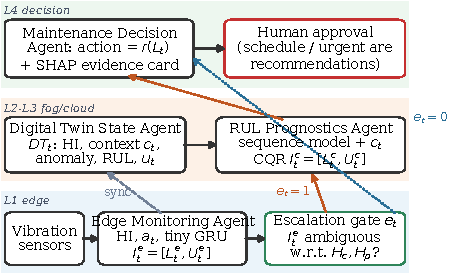
\includegraphics[width=\columnwidth]{figures/fig1_architecture.pdf}
\caption{HERA-PdM. The edge agent computes a calibrated RUL interval $I^e_t$; the gate escalates only if $I^e_t$ is not decision-sufficient; the fog/cloud agent uses the DT context $c_t$; schedule/urgent actions need human approval.}
\label{fig:arch}
\end{figure}

Fig.~\ref{fig:arch} shows the four layers. ``Agents'' are software components with fixed responsibilities and messages; no language model is used anywhere.

\textit{Edge Monitoring Agent.} Each vibration snapshot is reduced to $x_t\in\mathbb{R}^{28}$ (per axis: RMS, kurtosis, skewness, peak-to-peak, crest, impulse and shape factors, spectral centroid, six log band energies), z-scored against the asset's first snapshots and compressed by $\mathrm{sign}(z)\log(1{+}|z|)$. The health index is $h_t=\log(1+\frac1d\sum_j|z_{t,j}|)$; the anomaly score $a_t$ is the smoothed $h_t$ standardized by the asset's raw baseline, with alarm threshold $\tau_a$ at the 99th percentile of healthy training snapshots. A tiny model maps a short window to three RUL quantiles.

\textit{Digital Twin State Agent.} The twin is a synchronized state record $DT_t=\{$condition, sensor state, $h_t$, context $c_t$, $\hat R_t$, $I_t$, $u_t$, anomaly state$\}$ updated from a 12-byte sync $(t,h_t,a_t)$ per snapshot; $c_t\in\mathbb{R}^6$ holds fast/slow averages of $h_t$, their difference, running maximum, slope and cumulative excess over baseline. Absolute operating time is excluded because lifetimes vary by an order of magnitude.

\textit{RUL Prognostics Agent.} A sequence model $g_\phi$ maps a longer window $X_t$ and $c_t$ to non-crossing quantiles $(\hat q^{\,\alpha/2}_t,\hat q^{\,0.5}_t,\hat q^{\,1-\alpha/2}_t)$ trained with the pinball loss on $y_t=\min(\mathrm{RUL}_t,R_{\max})$.

\textit{Calibration (CQR-CV+).} The non-test assets are split into $K{=}4$ condition-balanced groups; inner model $g^{(-k)}$ is trained without group $k$, which yields out-of-fold scores $s_i=\max(\hat q^{\,\alpha/2}_i-y_i,\,y_i-\hat q^{\,1-\alpha/2}_i)$ for every non-test snapshot $i$ in group $k(i)$. Following CV+~\cite{barber2021jackknife} with CQR scores~\cite{romano2019cqr},
\begin{align}
L_t&=Q^{-}_{\alpha}\{\hat q^{\,\alpha/2,(-k(i))}_t-s_i\},\\
U_t&=Q^{+}_{1-\alpha}\{\hat q^{\,1-\alpha/2,(-k(i))}_t+s_i\},
\end{align}
where $Q^{-}_{\alpha}$ and $Q^{+}_{1-\alpha}$ are the $\lfloor\alpha(n{+}1)\rfloor$-th and $\lceil(1{-}\alpha)(n{+}1)\rceil$-th smallest values over the $n$ calibration snapshots; $\hat R_t$ is the mean inner median. CV+ guarantees coverage $\ge1-2\alpha$ (typically $\approx1-\alpha$) if assets are exchangeable; snapshots within an asset are dependent, so the guarantee is approximate and we test it. Split CQR on three held-out bearings is the baseline calibrator.

\textit{Decision and escalation.} With critical and planning horizons $\Hc$ and $\Hp$, the action of a value $v$ is $r(v)=$\,\textsc{urgent} if $v\le\Hc$, \textsc{schedule} if $\Hc<v\le\Hp$, else \textsc{continue}; the Maintenance Decision Agent acts on $\pi_t=r(L_t)$ (\textsc{continue} becomes \textsc{inspect} if $a_t>\tau_a$). \textsc{schedule}/\textsc{urgent} are recommendations with an explanation card (RUL, interval, anomaly evidence, top-3 SHAP~\cite{lundberg2017shap} contributors, rationale) that require approval. With $B=\{\Hc,\Hp\}$, the edge escalates if its interval is ambiguous or contradicts anomaly evidence:
\begin{equation}
e_t=\mathbb{I}\big[\exists h{\in}B{:}\,L^e_t{\le} h{<}U^e_t\big]\lor\mathbb{I}\big[a_t{>}\tau_a\wedge r(L^e_t){=}\mathrm{C}\big],
\end{equation}
where C denotes \textsc{continue}. A local \textsc{continue} needs $L^e_t>\Hp\ge\Hc$, so a critical asset ($y_t\le\Hc$) is left running locally only if $y_t\notin I^e_t$:
\begin{equation}
\Pr\big(e_t{=}0,\ \pi_t{=}\textsc{continue},\ y_t\le\Hc\big)\le\Pr(y_t\notin I^e_t),
\end{equation}
and false local \textsc{urgent} actions are bounded likewise. Unlike a width threshold, the gate ignores wide intervals inside one action region and escalates narrow ones crossing a boundary.

\textit{Cost model.} Payloads are counted in float32: always-cloud streams $x_t$ (112\,B/snapshot); HERA sends the 12\,B sync plus the untransmitted part of the window when $e_t{=}1$. Latency is edge time $+\,e_t(\mathrm{RTT}+$cloud time$)$ with an assumed RTT of \rttMs\,ms.

\begin{table}[t]
\centering
\caption{RUL accuracy and calibration on 17 held-out FEMTO bearings (4 bearing-grouped folds; mean$\pm$std over 3 seeds; RUL capped at 3000\,s; nominal coverage 90\%). Raw: uncalibrated quantiles; CQR: conformalized. $^\dagger$selected on calibration bearings.}
\label{tab:rul}
\setlength{\tabcolsep}{2.6pt}\footnotesize
\resizebox{\columnwidth}{!}{%
\begin{tabular}{lrcccccc}
\toprule
Model & Params & RMSE (s) & MAE (s) & Raw cov. & CQR cov. & MPIW (s) & CCE \\
\midrule
Edge-CNN & 2.7k & 1114$\pm$40 & 851$\pm$19 & 0.37 & 0.88$\pm$0.02 & 2080$\pm$120 & 0.035 \\
Edge-GRU$^\dagger$ & 2.5k & 816$\pm$30 & 525$\pm$65 & 0.69 & 0.84$\pm$0.04 & 1879$\pm$130 & 0.054 \\
\midrule
LSTM & 17.5k & 1200$\pm$79 & 778$\pm$69 & 0.53 & 0.86$\pm$0.04 & 2014$\pm$184 & 0.072 \\
LSTM+DT & 17.7k & 1202$\pm$127 & 824$\pm$119 & 0.44 & 0.86$\pm$0.01 & 1989$\pm$28 & 0.066 \\
GRU & 13.4k & 1149$\pm$95 & 706$\pm$87 & 0.54 & 0.85$\pm$0.03 & 2009$\pm$167 & 0.067 \\
GRU+DT & 13.6k & 1166$\pm$83 & 784$\pm$77 & 0.38 & 0.88$\pm$0.04 & 2145$\pm$244 & 0.051 \\
TCN & 16.8k & 1112$\pm$63 & 825$\pm$79 & 0.32 & 0.87$\pm$0.02 & 2122$\pm$170 & 0.032 \\
TCN+DT & 17.2k & 1047$\pm$77 & 808$\pm$49 & 0.31 & 0.89$\pm$0.02 & 2314$\pm$111 & 0.040 \\
CNN-LSTM & 15.3k & 1096$\pm$104 & 676$\pm$105 & 0.47 & 0.83$\pm$0.03 & 2147$\pm$104 & 0.044 \\
CNN-LSTM+DT$^\dagger$ & 15.7k & 1093$\pm$64 & 717$\pm$43 & 0.36 & 0.85$\pm$0.01 & 2008$\pm$75 & 0.062 \\
\midrule
LSTM+DT (MSE) & -- & 1288$\pm$64 & 945$\pm$76 & -- & -- & -- & -- \\
GRU+DT (MSE) & -- & 1298$\pm$88 & 959$\pm$117 & -- & -- & -- & -- \\
TCN+DT (MSE) & -- & 1114$\pm$26 & 879$\pm$25 & -- & -- & -- & -- \\
CNN-LSTM+DT (MSE) & -- & 1100$\pm$66 & 789$\pm$45 & -- & -- & -- & -- \\
\bottomrule
\end{tabular}}
\end{table}

\begin{table}[t]
\centering
\caption{Hierarchical policies, ablations and system cost (all 17 bearings, mean$\pm$std over 3 seeds). Esc.: escalated snapshots; Unsafe: critical snapshots ($y{\le}H_c$) left without maintenance action; FM: false maintenance on healthy snapshots ($y{>}H_p$); B/s: payload bytes per snapshot; Lat.: mean decision latency with an assumed 50\,ms RTT. $^\ddagger$escalation budget matched to HERA on calibration bearings.}
\label{tab:policies}
\setlength{\tabcolsep}{2.2pt}\footnotesize
\resizebox{\columnwidth}{!}{%
\begin{tabular}{lcccccc}
\toprule
Policy & Esc.\,(\%) & Unsafe\,(\%) & FM\,(\%) & RMSE\,(s) & B/s & Lat.\,(ms) \\
\midrule
Always-edge & 0.0 & 6.7$\pm$5.9 & 86.8$\pm$15.4 & 809 & 0 & 0.1 \\
Always-cloud & 100.0 & 5.4$\pm$1.3 & 84.0$\pm$5.6 & 1090 & 112 & 50.2 \\
Cloud point + fixed thr. & 100.0 & 41.0$\pm$3.4 & 23.6$\pm$1.4 & 1100 & 112 & 50.2 \\
\midrule
\textbf{HERA-full} & 87.5 & 9.4$\pm$3.7 & 75.0$\pm$11.6 & 1083 & 117 & 44.1 \\
HERA w/o anomaly term & 87.4 & 9.6$\pm$3.8 & 75.0$\pm$11.6 & 1084 & 117 & 44.0 \\
HERA-no-DT & 87.5 & 6.5$\pm$5.7 & 82.6$\pm$11.2 & 1088 & 117 & 44.1 \\
\midrule
HERA-no-UQ (point margin) & 32.7 & 48.2$\pm$5.5 & 17.0$\pm$4.4 & 1014 & 69 & 16.5 \\
HERA-fixed (anomaly trig.) & 3.9 & 6.7$\pm$5.7 & 86.8$\pm$15.4 & 811 & 27 & 2.1 \\
\midrule
Width gate$^\ddagger$ & 87.4 & 9.5$\pm$3.8 & 75.0$\pm$11.6 & 1084 & 117 & 44.0 \\
Linear score gate$^\ddagger$ & 88.9 & 7.6$\pm$2.1 & 77.0$\pm$10.6 & 1086 & 117 & 44.8 \\
Random gate$^\ddagger$ & 85.2 & 6.1$\pm$0.9 & 81.8$\pm$4.7 & 1059 & 124 & 42.9 \\
\bottomrule
\end{tabular}}
\end{table}

\begin{figure}[t]
\centering
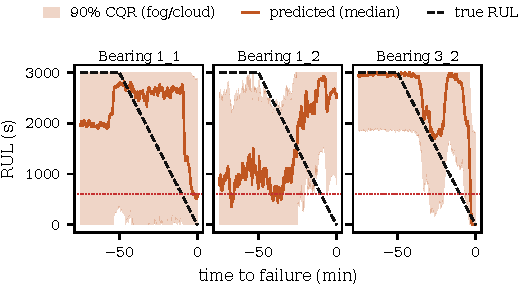
\includegraphics[width=\columnwidth]{figures/fig3_trajectories.pdf}
\caption{Fog/cloud median RUL and 90\% CQR-CV+ interval before failure (seed 0; per dataset the test bearing with most degradation-phase snapshots). Dotted line: $\Hc$.}
\label{fig:traj}
\end{figure}
\begin{figure*}[t]
\centering
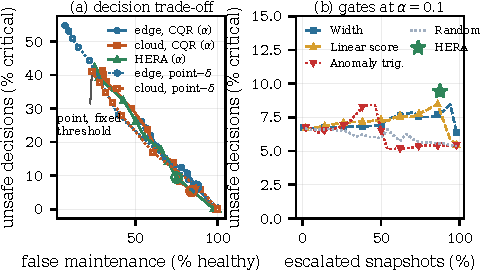
\includegraphics[width=\textwidth]{figures/fig4_tradeoff.pdf}
\caption{(a,c) Unsafe decisions vs.\ false maintenance when sweeping $\alpha$ (calibrated; circles at $\alpha{=}0.1$) or a margin $\delta$ (point). (b,d) Unsafe decisions vs.\ escalation budget for gates on the same $\alpha{=}0.1$ edge intervals; green line: HERA with $\alpha_e$ swept.}
\label{fig:tradeoff}
\end{figure*}

\section{Experimental Setup}
\textit{Data.} FEMTO-ST/PRONOSTIA~\cite{nectoux2012pronostia}: \feNBearings{} bearings under three conditions, 0.1\,s snapshots every 10\,s (\feNSnap{} snapshots), full test trajectories; several bearings fail abruptly. XJTU-SY~\cite{wang2020xjtu}: \xjNBearings{} bearings under 35\,Hz/12\,kN, 37.5\,Hz/11\,kN and 40\,Hz/10\,kN, 1.28\,s snapshots every minute (\xjNSnap{} snapshots), mostly gradual degradation. RUL caps are $R_{\max}{=}\feRmax$\,s (FEMTO) and \xjRmax\,s (XJTU-SY); $\Hc{=}0.2R_{\max}$, $\Hp{=}0.6R_{\max}$; windows are 16/64 and 8/32 snapshots (edge/cloud). SCANIA Component X~\cite{kharazian2025scania} (dataset DOI 10.5878/bnh5-ka77, CC BY 4.0): \flN{} trucks with irregular operational readouts (counters and histograms), \flNf{} with an in-study repair and the rest right-censored; we use it only for unit-level alarm timing (Sec.~\ref{sec:fleet}).

\textit{Protocol.} Condition-balanced bearing-grouped folds (\feNFolds{} for FEMTO, \xjNFolds{} for XJTU-SY) test every bearing once. Each architecture's hyper-parameters (width 32--128, 8 or 25 epochs, input noise) and the edge/cloud architecture choice were selected on inner validation bearings from training bearings only (FEMTO: \feEdgeModel/\feCloudModel+DT; XJTU-SY: \xjEdgeModel/\xjCloudModel+DT). Three seeds per model; metrics are pooled over test bearings and reported as mean$\pm$std; paired Wilcoxon tests use bearings as units.

\textit{Baselines and metrics.} LSTM, GRU, TCN~\cite{bai2018tcn} and CNN-LSTM with and without DT context, MSE point models; always-edge, always-cloud and point-with-fixed-threshold policies; ablations without uncertainty (point margin), DT or anomaly term; anomaly-trigger (as in~\cite{saleh2026hama}), width (confidence-style deferral), linear-score and random gates at HERA's budget. We report RMSE, MAE, coverage (Cov.), mean interval width (MPIW), \emph{unsafe rate} (critical snapshots with \textsc{continue}/\textsc{inspect}), false maintenance (FM, \textsc{schedule}/\textsc{urgent} when $y_t>\Hp$), escalation, payload, latency (single-thread host CPU, Apple M2 Pro; no energy measured) and, per bearing, the timing of the first sustained maintenance alarm.


\section{Results and Discussion}
\textit{RQ1: accuracy.} Table~\ref{tab:rul} shows opposite regimes. On FEMTO, the \feEdgeParams-parameter edge model was most accurate (RMSE \feRmseEdge\,s with CQR-CV+ vs.\ \feRmseCloud\,s for \feCloudModel+DT), because abrupt failures leave larger models nothing to exploit. On XJTU-SY, fog/cloud models were clearly better (best split-trained \xjBestCloudRmse\,s, \xjBestCloudModel) than the selected edge model (\xjRmseEdgeSplit\,s). DT context lowered RMSE for \feDtHelps{} of 4 architectures on FEMTO but only \xjDtHelps{} on XJTU-SY; cross-fitted ensembles (CV+) also improved point accuracy.



\input{tables/table4_timing.tex}

\textit{RQ2: calibration.} Split CQR with three calibration bearings under-covered on FEMTO (\feSplitCovMin--\feSplitCovMax). CQR-CV+, which calibrates on all non-test bearings, reached \fePicpEdge{} (edge) and \fePicpCloud{} (cloud) on FEMTO and \xjPicpCloud--\xjPicpEdge{} on XJTU-SY, at the price of wider intervals (MPIW \feMpiwEdge\,s and \xjMpiwCloud\,s). Per-bearing coverage still varied strongly (lowest cloud coverage \feCovMinCloud{} and \xjCovMinCloud), so exchangeability between bearings remains the binding assumption. Fig.~\ref{fig:traj} shows intervals narrowing once degradation is visible, far earlier on XJTU-SY.



\textit{RQ4: unsafe decisions.} Point estimates with fixed thresholds left \feUnsafePoint\% (FEMTO) and \xjUnsafePoint\% (XJTU-SY) of critical snapshots without a maintenance action, versus \feUnsafeHera\% and \xjUnsafeHera\% for HERA (Table~\ref{tab:policies}); the differences were \feCiUnsafePt{} (FEMTO) and \xjCiUnsafePt{} (XJTU-SY) over bearings (Wilcoxon $p$\,\fePHeraPoint, $p{=}$\xjPHeraPoint), and false maintenance rose by \feCiFmPt{} and \xjCiFmPt. Sweeping $\alpha$ or a point margin $\delta$ (Fig.~\ref{fig:tradeoff}a,c) shows that calibrated and margin-adjusted point policies lie close to one frontier: calibration contributes a principled, held-out choice of operating point rather than better attainable decisions.


\textit{RQ3 and RQ5: escalation and system trade-off.} On FEMTO, 90\% edge intervals (\feMpiwEdge\,s on a \feRmax\,s range) almost always straddled $\Hp$, so HERA escalated \feEscHera\% of snapshots, sent more payload than always-cloud streaming (\feBytesHera{} vs.\ \feBytesCloud\,B) and gave no decision benefit. On XJTU-SY, HERA escalated \xjEscHera\%, matched always-cloud safety (\xjUnsafeHera\% vs.\ \xjUnsafeCloud\%) with lower false maintenance (\xjFmHera\% vs.\ \xjFmCloud\%), better RMSE (\xjRmsePolHera{} vs.\ \xjRmsePolCloud\,s), \xjBytesHera{} instead of \xjBytesCloud\,B/snapshot and mean latency \xjLatHera{} vs.\ \xjLatCloud\,ms. Two caveats temper this: the FM difference to always-cloud (\xjCiFmCl) comes from the two long-lived condition-3 bearings and its interval reaches zero, and the edge-only calibrated policy traced a better frontier than HERA (Fig.~\ref{fig:tradeoff}c) because the conservative edge intervals rarely under-predict. At matched budget, the width gate gave identical results (\xjUnsafeWidth\%/\xjFmWidth\%) and the linear-score gate nearly so (Fig.~\ref{fig:tradeoff}b,d); the anomaly trigger escalated only \xjEscHeraFixed\% (anomaly AUROC \feDetAnomAuroc/\xjDetAnomAuroc). Relaxing $\alpha_e$ to 0.3 reduced escalation to \feEscAlphaThirty\%/\xjEscAlphaThirty\% while unsafe decisions rose to \feUnsafeAlphaThirty\%/\xjUnsafeAlphaThirty\%. Removing the DT context lowered FM on XJTU-SY (\xjFmHeraNoDT\%) at higher unsafe rate (\xjUnsafeHeraNoDT\%), so the DT context is not uniformly beneficial.


\textit{Per-bearing timing and sensitivity.} Table~\ref{tab:timing} exposes the main practical limitation: because the 90\% lower bound falls below $\Hp$ early, every calibrated policy raised its first sustained maintenance alarm while the true RUL still exceeded $R_{\max}$ for \fePremHera{} of \feNBearings{} FEMTO and \xjPremHera{} of \xjNBearings{} XJTU-SY bearings, whereas the point policy was late for \feLatePoint{} and \xjLatePoint{} bearings. Neither is acceptable for scheduling; per-snapshot marginal coverage is the wrong target for alarm timing. In all five horizon settings and all four halved/doubled-$R_{\max}$ runs, HERA left fewer critical snapshots without action than the point policy; with a halved cap on XJTU-SY, HERA reached low false maintenance at the always-cloud unsafe rate (Table~\ref{tab:timing}).

\textit{Bearing-level risk control.} We also calibrated the alarm offset directly for timing: an onset-gated two-stage alarm whose offset $\lambda$ was chosen by conformal risk control~\cite{angelopoulos2024crc} on the CV+ out-of-fold predictions of the non-test bearings, so that $\Pr(\text{late or missing alarm})\le\varepsilon$ per bearing. At $\varepsilon{=}0.1$ the held-out late rate stayed within the target (\feLateCrcTen\% FEMTO, \xjLateCrcTen\% XJTU-SY vs.\ \feLatePointHp\% and \xjLatePointHp\% for the point policy), but only by alarming early: \fePremCrcTen\% and \xjPremCrcTen\% of alarms were premature and the onset gate escalated \feEscCrcTen\% and \xjEscCrcTen\% of snapshots. The reason is a heavy tail of required offsets: the median bearing needed an offset of \feReqOffMed{} (FEMTO) and \xjReqOffMed{} (XJTU-SY) of $R_{\max}$ to be warned in time, but the two least predictable bearings needed \feReqOffTop{} and \xjReqOffTop. This is a sample-size effect:

\textit{Proposition 1.} Let a fraction $\pi$ of $n$ calibration units be late for every admissible offset (no usable warning). CRC with the binary lateness loss returns a non-trivial offset at level $\varepsilon$ only if $(n\pi+1)/(n+1)\le\varepsilon$, i.e.\ $\pi<\varepsilon$ and $n\ge(1-\varepsilon)/(\varepsilon-\pi)$.

\textit{Proof.} The empirical risk of every offset is at least $\pi$, and CRC requires $(n\hat R+1)/(n+1)\le\varepsilon$~\cite{angelopoulos2024crc}. $\square$

For $\varepsilon{=}0.1$ and $\pi{=}0.05$ this needs $n\ge\nMinTenFive$, beyond the $\approx$12 bearings per fold available here; below it CRC must alarm at the earliest possible offset.

\input{tables/table7_fleet.tex}

\textit{Fleet-scale validation.}\label{sec:fleet} To test Proposition~1 where $n$ is large, we applied the same unit-level CRC to \flN{} Scania trucks: a logistic-regression edge model and a gradient-boosted cloud model (vehicle-grouped 5-fold cross-fitting, AUROC \flAucEdge{} and \flAucCloud) score $\Pr(\mathrm{RUL}\le\Hp)$ per readout with $\Hc{=}12$ and $\Hp{=}48$ time units; alarms need two consecutive readouts; HERA opens a latched edge gate at half the cloud threshold. Table~\ref{tab:fleet} averages 50 random calibration/test splits. Fixed thresholds were late for \flFixEdLate\% (edge) and \flFixClLate\% (cloud) of failing trucks, whereas CRC hit its target (\flClBigLate\% at $\varepsilon{=}0.1$, \flHeFiveLate\% at 0.05, \flHeTwentyLate\% at 0.2). Growing the calibration fleet from 12 to 1000 failing trucks tightened the 95th-percentile late rate from \flClSmallLateQ\% to \flClBigLateQ\% and lowered false alarms from \flClSmallFa\% to \flClBigFa\%. HERA matched always-cloud decisions (\flHeBigLate\%/\flHeBigFa\% vs.\ \flClBigLate\%/\flClBigFa\%) while escalating only \flHeBigEsc\% of readouts; the edge model alone was almost as good (\flEdBigFa\% false alarms) because the cloud model was not more accurate. False alarms stayed high because the failure signal is weak.

\begin{table}[t]
\centering
\caption{Top: detection of imminent failure (RUL $\le H_c$) per snapshot, thresholds set on training data (mean over 3 seeds). Bottom: compute of the selected edge and fog/cloud models (host CPU, 1 thread, batch 1).}
\label{tab:detect}
\footnotesize\setlength{\tabcolsep}{2.4pt}
\begin{tabular}{l|ccc|ccc}
\toprule
 & \multicolumn{3}{c|}{FEMTO} & \multicolumn{3}{c}{XJTU-SY} \\
Detector & Prec. & Rec. & AUROC & Prec. & Rec. & AUROC \\
\midrule
Anomaly score $a_t$ & 0.27 & 0.26 & 0.81 & 0.21 & 0.34 & 0.80 \\
Isolation Forest & 0.27 & 0.15 & 0.77 & 0.15 & 0.13 & 0.81 \\
Edge interval $L^e_t\le H_c$ & 0.07 & 0.68 & 0.70 & 0.06 & 0.94 & 0.82 \\
Cloud interval $L^c_t\le H_c$ & 0.05 & 0.82 & 0.65 & 0.17 & 0.76 & 0.81 \\
\midrule
Model & Params & MACs & ms & Params & MACs & ms \\
\midrule
Edge model & 2.5k & 0.03M & 0.15 & 2.7k & 0.02M & 0.07 \\
Cloud model & 62.1k & 3.61M & 1.11 & 13.6k & 0.38M & 0.62 \\
\bottomrule
\end{tabular}
\end{table}


\textit{Detection and compute.} Table~\ref{tab:detect} shows why no simple trigger suffices: the edge anomaly score reached AUROC \feDetAnomAuroc{} and \xjDetAnomAuroc{} but recall of only \feDetAnomRec{} and \xjDetAnomRec{} at its training-calibrated threshold, whereas the calibrated lower bounds recalled \feDetEdgeLBRec--\xjDetEdgeLBRec{} of critical snapshots at low precision, the safety/false-alarm trade-off seen in Fig.~\ref{fig:tradeoff}. The edge models need tens of thousands of MACs and well under a millisecond; the fog/cloud models need roughly 20--120 times more MACs. Run unchanged in an ARM64 Linux container capped at one CPU and 1\,GB (Apple M2 Pro host, not embedded hardware), the exported models reproduced host outputs to below \armParity{} and took at most \armEdgeMs\,ms (edge) and \armCloudMs\,ms (cloud) per window, plus \armFeatMs\,ms for feature extraction, with \armRss\,MB peak memory; with the container pinned to one core, p99 stayed below \armPinP\,ms.

\textit{Explainability and oversight.} Expected-gradient SHAP on 300 degradation-phase snapshots ranked low-frequency band energies and the spectral centroid (FEMTO) and the DT fast health-index average and mid- and high-frequency band energies (XJTU-SY) highest; additivity errors were \feShapRel\% and \xjShapRel\% of the explained deviation. An automatically generated card (FEMTO) reads:

\smallskip\noindent\fbox{\parbox{0.96\columnwidth}{\footnotesize \textbf{Asset} Bearing1\_3, snapshot 2078. \textbf{RUL} 578\,s, 90\% interval [0, 2138]\,s. \textbf{Anomaly} $a_t$=15.8 (threshold 17.04, no alarm). \textbf{Top SHAP} h\_band0\_1k (-1489\,s), v\_band2\_4k (-1244\,s), h\_centroid (+1175\,s). \textbf{Recommendation} urgent maintenance --- \emph{requires human approval}. \textbf{Rationale} lower bound 0\,s $\le H_{\mathrm{c}}$.}}

\smallskip

\noindent All fields come from the predictors via a fixed template. Approval requests covered \feApprHera\% (FEMTO) and \xjApprHera\% (XJTU-SY) of HERA snapshots, an operator load that shows calibrated but wide intervals shift burden to humans.

\begin{table}[t]
\centering
\caption{Deployment guide derived from the measured results (FEMTO / XJTU-SY).}
\label{tab:guide}
\footnotesize\setlength{\tabcolsep}{2pt}
\begin{tabular}{@{}>{\raggedright\arraybackslash}p{1.75cm}>{\raggedright\arraybackslash}p{1.95cm}>{\raggedright\arraybackslash}p{4.3cm}@{}}
\toprule
Plant condition & Recommended policy & Evidence \\
\midrule
Safety-critical, any fleet & Decide on calibrated lower bound & unsafe \feUnsafeHera\%/\xjUnsafeHera\% vs.\ \feUnsafePoint\%/\xjUnsafePoint\% for point thresholds \\
Degradation visible early & Uncertainty-gated escalation & XJTU-SY: same unsafe rate as always-cloud, FM \xjFmHera\% vs.\ \xjFmCloud\% (CI reaches 0) \\
Abrupt, warning-free failures & Always-edge calibrated & FEMTO: HERA escalated \feEscHera\%, no benefit; edge RMSE \feRmseEdge\,s best \\
Limited bandwidth & Gate on interval width & width gate equal to decision-sufficiency gate on both datasets \\
Alarm-timing guarantee needed & Conformal risk control with enough units (Prop.~1) & bearings ($\approx$12 units): premature \fePremCrcTen\%/\xjPremCrcTen\%; trucks (1000): late \flHeBigLate\% at target 10\% \\
Limited operator capacity & Relax $\alpha$ or add onset detection & approval load \feApprHera\%/\xjApprHera\% at $\alpha{=}0.1$ \\
\bottomrule
\end{tabular}
\end{table}

\textit{Lessons for deployment.} Table~\ref{tab:guide} condenses the evidence. (i)~\emph{Calibrate before routing}: calibrated intervals removed most unsafe point-threshold decisions on both datasets. (ii)~\emph{Hierarchy pays only if degradation is observable early}: escalation helped on XJTU-SY and not on FEMTO. (iii)~\emph{Small fleets strain calibration}: three calibration bearings under-covered, cross-fitting on all assets fixed pooled coverage, and per-asset coverage still varied. (iv)~\emph{The interval width matters more than the gate}: decision-sufficiency and width gates coincided. (v)~\emph{Unit-level guarantees need fleets}: with a dozen units risk control alarms early (Proposition~1); with a thousand trucks it met its target. (vi)~\emph{Wide intervals move work to humans}: approval load, not model accuracy, limits human-centric use. Limitations: 32 bearings, approximate exchangeability, a state-based DT, no timing on embedded hardware, analytic communication, and no deployment or user study.

\section{Conclusion}
Cross-fitted conformal RUL intervals removed most unsafe decisions of point-threshold maintenance on two bearing datasets. Using them to gate edge-to-cloud escalation paid off on gradually degrading bearings and on a truck fleet, where HERA matched always-cloud safety with a fraction of the cloud traffic, but not under abrupt failures; the specific decision-sufficiency rule was no better than a width gate. Calibrating alarm timing with conformal risk control is feasible only with enough units (Proposition~1): with a dozen bearings it alarmed early, whereas on \flN{} trucks it met its lateness target, at a false-alarm cost set by the weak failure signal. Better early-warning features are therefore the next lever, not routing rules.

\bibliographystyle{IEEEtran}
\bibliography{references}

\end{document}
